% Source: graduate-coursework/Research/Intro_to_Agents/handouts/Part7_Parallelization.tex

\documentclass[border=4pt]{standalone}
\usepackage{amsmath,amssymb,amsfonts}
\usepackage[T1]{fontenc}
\usepackage{graphicx}
\usepackage{lmodern}
\usepackage{tikz}
\usepackage{xcolor}
\usetikzlibrary{shapes.geometric, arrows.meta, positioning, calc, fit, backgrounds, matrix, decorations.pathreplacing}

\definecolor{UofSCGarnet}{HTML}{73000a}
\definecolor{UofSCBlack}{HTML}{000000}
\definecolor{UofSCWhite}{HTML}{ffffff}
\definecolor{UofSCRose}{HTML}{CC2E40}
\definecolor{UofSCAtlantic}{HTML}{466A9F}
\definecolor{UofSCCongaree}{HTML}{1F414D}
\definecolor{UofSCHorseshoe}{HTML}{65780B}
\definecolor{UofSCGrass}{HTML}{CED318}
\definecolor{UofSCHoneycomb}{HTML}{A49137}
\definecolor{UofSC90Black}{HTML}{363636}
\definecolor{UofSC70Black}{HTML}{5C5C5C}
\definecolor{UofSC50Black}{HTML}{A2A2A2}
\definecolor{UofSCWarmGrey}{HTML}{676156}
\definecolor{UofSCSandstorm}{HTML}{FFF2E3}
\definecolor{UofSCDarkGarnet}{HTML}{570008}
\definecolor{UofSCAzalea}{HTML}{844247}

\tikzset{
    % Node styles - all with sharp corners
    agentbox/.style={
        rectangle,
        draw=UofSCGarnet,
        fill=UofSCSandstorm,
        thick,
        minimum width=2cm,
        minimum height=0.8cm,
        text centered,
        font=\footnotesize
    },
    processbox/.style={
        rectangle,
        draw=UofSCAtlantic,
        fill=UofSCWhite,
        thick,
        minimum width=2.5cm,
        minimum height=0.7cm,
        text centered,
        font=\footnotesize
    },
    syncbox/.style={
        rectangle,
        draw=UofSCCongaree,
        fill=UofSCCongaree!20,
        thick,
        minimum width=3cm,
        minimum height=0.5cm,
        text centered,
        font=\footnotesize\bfseries
    },
    resultbox/.style={
        rectangle,
        draw=UofSCHorseshoe,
        fill=UofSCGrass!30,
        thick,
        minimum width=2cm,
        minimum height=0.7cm,
        text centered,
        font=\footnotesize
    },
    % Arrow styles
    myarrow/.style={
        ->,
        >=Stealth,
        thick,
        UofSCBlack
    },
    dashedarrow/.style={
        ->,
        >=Stealth,
        thick,
        dashed,
        UofSC70Black
    },
    % Timeline styles
    timeline/.style={
        draw=UofSCBlack,
        thick,
        ->,
        >=Stealth
    },
    timeblock/.style={
        rectangle,
        draw=none,
        minimum height=0.5cm,
        text centered,
        font=\tiny
    }
}

\begin{document}
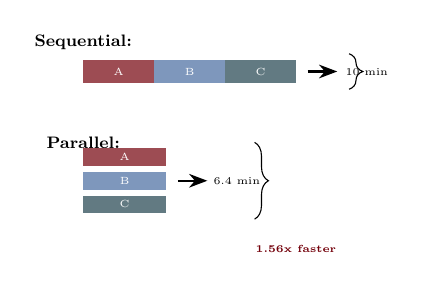
\begin{tikzpicture}[scale=0.75, transform shape]
                % Sequential execution
                \node[font=\footnotesize\bfseries] at (0,2.5) {Sequential:};
                \fill[UofSCGarnet!70] (0,1.8) rectangle (1.2,2.2);
                \fill[UofSCAtlantic!70] (1.2,1.8) rectangle (2.4,2.2);
                \fill[UofSCCongaree!70] (2.4,1.8) rectangle (3.6,2.2);
                \node[font=\tiny,white] at (0.6,2) {A};
                \node[font=\tiny,white] at (1.8,2) {B};
                \node[font=\tiny,white] at (3.0,2) {C};
                \draw[myarrow] (3.8,2) -- (4.3,2);
                \node[font=\tiny] at (4.8,2) {10 min};

                % Parallel execution
                \node[font=\footnotesize\bfseries] at (0,0.8) {Parallel:};
                \fill[UofSCGarnet!70] (0,0.4) rectangle (1.4,0.7);
                \fill[UofSCAtlantic!70] (0,0) rectangle (1.4,0.3);
                \fill[UofSCCongaree!70] (0,-0.4) rectangle (1.4,-0.1);
                \node[font=\tiny,white] at (0.7,0.55) {A};
                \node[font=\tiny,white] at (0.7,0.15) {B};
                \node[font=\tiny,white] at (0.7,-0.25) {C};
                \draw[myarrow] (1.6,0.15) -- (2.1,0.15);
                \node[font=\tiny] at (2.6,0.15) {6.4 min};

                % Speedup annotation
                \draw[decorate,decoration={brace,amplitude=5pt,mirror}] (4.5,1.7) -- (4.5,2.3);
                \draw[decorate,decoration={brace,amplitude=5pt,mirror}] (2.9,-0.5) -- (2.9,0.8);
                \node[font=\tiny\bfseries,UofSCGarnet] at (3.6,-1) {1.56x faster};
            \end{tikzpicture}
\end{document}
